\chapter{Rezultati}
\section{Točnost razvrščanja}
Pri interpretaciji točnosti razvrščanja stanj je potrebno upoštevati, da razvrščamo tri različna stanja, zato so že rezultati okoli 50\% bistveno nad nivojem naključnosti, ki je v primeru treh različnih stanj 33\%.
\section{Delitev podatkov}
Za končno raziskavo smo izbrali posnetke serij 3, 7 in 11 iz MMID. Vsaka serija vsebuje 109 posnetkov, vsak posnetek 30 primerov stanj, vse skupaj smo jih pridobili 9854. Primere stanj smo skrčili na enakomerno razporeditev z 2456 primeri vsakega stanja. Sami smo posneli nekaj minut posnetkov. Posneli smo vsega skupaj 250 primerov stanj, ki smo jih skrčili na enakomerno razporeditev, 62 primerov vsakega stanja. Za učenje nevronskih mrež smo uporabljali množice za učenje s 75\% podatkov in množice za testiranje s 25\% podatkov. Podatki so bili naključno razporejeni med učno in testno množico. Ker smo podatke delili naključno, se lahko različni posnetki stanj istega prostovoljca pojavijo v učni in testni množici. Pri dodatnem učenju mreže smo uporabili posnetke ene osebe za učenje in testiranje. To skupaj pomeni, da sistem ne deluje medosebno.


\section{Rezultati na MMID}
Za izbiro metode povezljivosti, načina filtriranja, dolžine epohe in frekvenčnega pasu smo uporabili podatkovno zbirko MMID.

\subsection{Izbira metode povezljivosti}
Ker je kompleksni Pearsonov korelacijski koeficient izračunan iz analitičnih signalov, ga lahko definiramo samo za ozke frekvenčne pasove. Pri računanju Grangerjevega indeksa vzročnosti te omejitve ni, zato smo ga lahko računali na celotnem frekvenčnem območju do 45Hz. Prav tako se je pojavilo vprašanje kako dolgo epoho EEG signala bomo potrebovali za uspešno razvrščanje. Kot možnosti smo vzeli prvo sekundo, prvi dve sekundi, drugi dve sekundi in prve štiri sekunde po dogodku. Točnost razvrščanja smo ocenili z zgoraj navedeno nevronsko mrežo. Za najboljšo metodo se je izkazal kompleksni Pearsonov korelacijski koeficient na območju 13-20 Hz z najdaljšimi epohami, 4s. Celotno območje primerjav je razvidno iz slike \ref{slika:primerjava_obmocij}.
\begin{figure}
    \begin{center}
    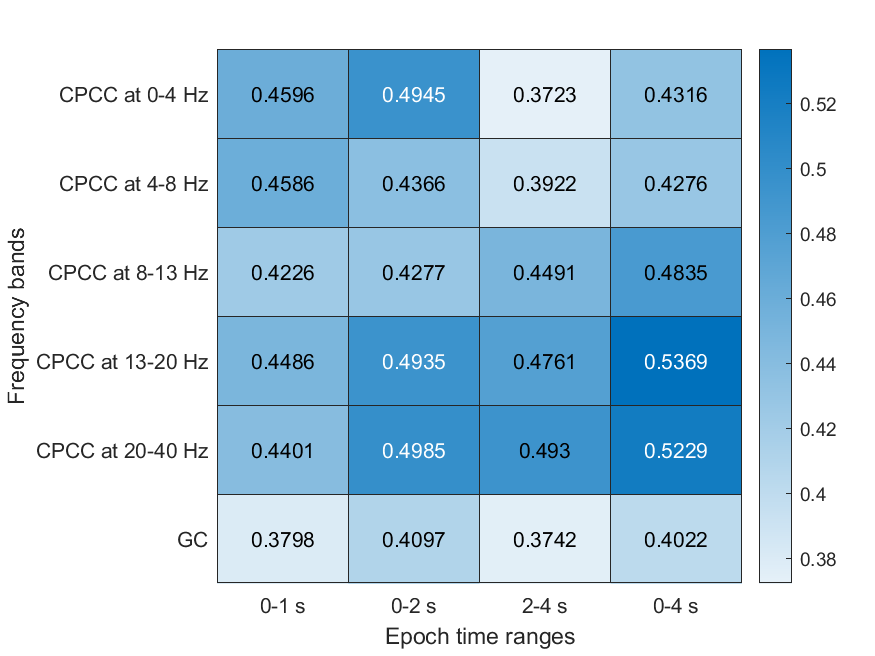
\includegraphics[width=1\linewidth]{slike/Comparison.png}
    \end{center}
    \caption[Točnost razvrščanja po frekvenčnih območjih in dolžini epoh.]{Točnost razvrščanja po frekvenčnih območjih in dolžini epoh za CPCC in GC. Od zgoraj navzdol: CPCC po pasovih delta, theta, alpha, beta in gamma. Spodnja vrstica: Grangerjev indeksa vzorčnosti. Epohe od leve proti desni: prva sekunda, prvi dve sekundi, drugi dve sekundi, prve štiri sekunde.}
    \label{slika:primerjava_obmocij}
\end{figure}

\newpage
\subsection{Izbira uporabljenih filtrov}
Knjižnica EEGLAB vsebuje samo filtre z ničelno fazo, ki filtrirajo naprej in nato nazaj po času, kar v našem primeru ni primerno, saj podatke prejemamo sekvenčno. Filtrov z ničelno fazo ni mogoče uporabiti v realnem času. Podatke smo želeli filtrirati s pomočjo Butterworthovega filtra, ki vsebuje stanja. Stanja nam omogočajo filtriranje sekvenčnih podatkov saj preprečijo napako na začetku filtra kjer le-ta potrebuje predpostaviti začetno staje vseh signalov 0. Ker filtra nista enakovredna, saj prvi ne spreminja faz drugi pa jih zamakne, uporabljena metoda CPCC pa deluje na zamikih faz, smo izvedli dodatno testiranje, da bi preverili ali pristop deluje enako učinkovito. Razvrščanje matrik, pridobljenih z Butterwothovim filtrom (slika \ref{slika:filter_matrika}b) v primerjavi z filtrom z ničelno fazo (slika \ref{slika:filter_matrika}a) je bilo primerljivo točno za frekvenčni pas beta (slika \ref{slika:primerjava_filtrov}) iz česar lahko sklepamo, da je filtriranje z Butterworthovim filtrom primerno.
\begin{figure}
    \begin{center}
    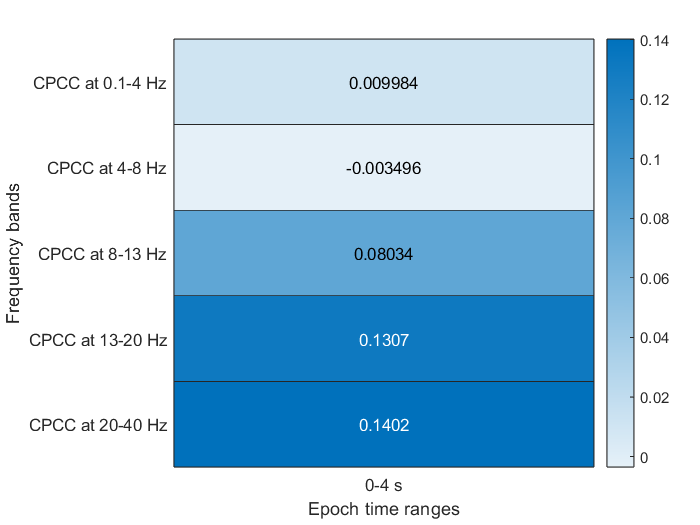
\includegraphics[width=1 \linewidth]{slike/ComparisonFilters.png}
    \end{center}
    \caption[Točnost razvrščanja glede na tip filtra in frekvenčno območje.]{Primerjava točnosti razvrščanja glede na tip filtra. Uporabljena metoda CPCC za epoho prvih štirih sekund za frekvenčne pasove delta, theta, alpha, beta in gamma. Razvrščanje z zgoraj navedeno nevronsko mrežo. Modra predstavlja Butterwothov filter, oranžna predstavlja filter z ničelno fazo.}
    \label{slika:primerjava_filtrov}
\end{figure}

\begin{figure}
    \begin{center}
    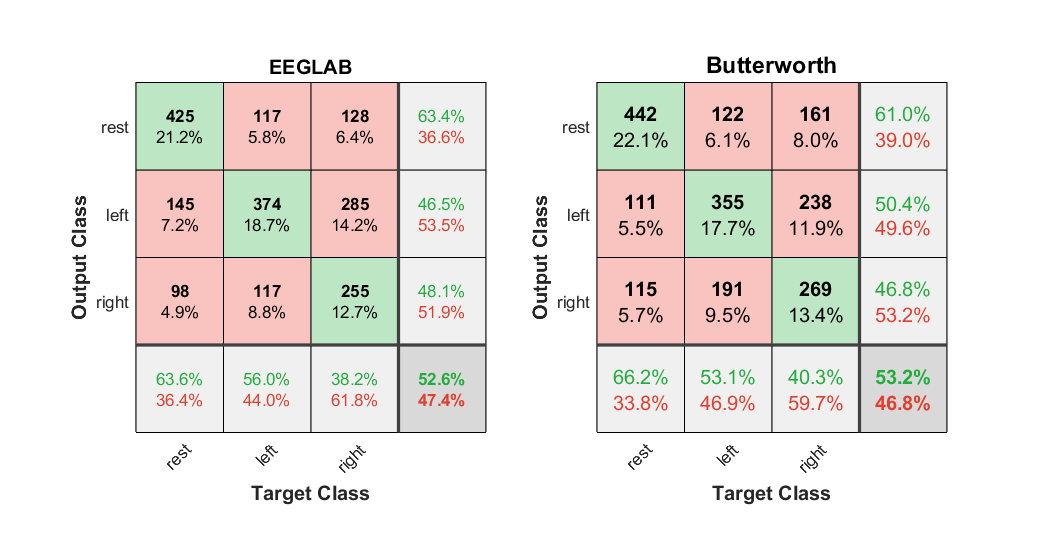
\includegraphics[width=1\linewidth]{slike/ComparisonFilters2.png}
    \end{center}
    \caption[Matriki zmede nevronskih mrež za frekvenčno območje beta.]{Matriki zmede nevronskih mrež, naučenih na podatkih, filtriranih s filtrom z ničelno fazo (levo) in Butterworthovim filtrom (desno). Uporabljena metoda CPCC za epoho prvih štirih sekund za frekvenčni pas beta. V zelenih poljih vidna točnost za posamezna stanja. Od zgoraj navzdol: stanje mirovanja, skrčena leva pest, skrčena desna pest.}
    \label{slika:filter_matrika}
    \end{figure}

\subsection{Rezultati z okoljem Classification Learner}
Z uporabo aplikacije Clasifiacation Learner smo testirali več načinov razvrščanja. Iz rezultatov predstavljenih v tabeli \ref{tabela:primerjava_tocnosti} lahko razberemo, da so se za najbolj uspešne izkazale metode podpornih vektorjev (SVM), vendar so te metode računsko zahtevne, kar otežuje izvedbo v realnem času. Dober kandidat bi lahko bila odločitvena drevesa, saj so enostavna za učenje in interpretacijo, vendar so le ta dosegla 41\% točnost. Nevronske mreže ki jih podpira aplikacija so enostavne, vendar pa je njihova interpretacija težja.  Dosegle so 49\% točnost.
\begin{table}
\centering
\begin{tabular}{|l|l|c|}
\hline
vrsta razvrščanja & metoda & točnost [\%] \\
\hline SVM&Quadratic SVM&53\\
\hline SVM&Linear SVM&53\\
\hline SVM&Medium Gaussian SVM&53\\
\hline Ensemble&Subspace Discriminant&53\\
\hline SVM&Cubic SVM&52\\
\hline Kernel&SVM Kernel&52\\
\hline Kernel&Logistic Regression Kernel&52\\
\hline SVM&Coarse Gaussian SVM&50\\
\hline Efficient Logistic Regression&Efficient Logistic Regression&49\\
\hline Neural Network&Wide Neural Network&49\\
\hline Neural Network&Medium Neural Network&47\\
\hline Efficient Linear SVM&Efficient Linear SVM&46\\
\hline Neural Network&Trilayered Neural Network&45\\
\hline Neural Network&Bilayered Neural Network&45\\
\hline Naive Bayes&Kernel Naive Bayes&45\\
\hline Neural Network&Narrow Neural Network&45\\
\hline Ensemble&Bagged Trees&44\\
\hline KNN&Coarse KNN&44\\
\hline Ensemble&Boosted Trees&43\\
\hline Ensemble&RUSBoosted Trees&42\\
\hline Tree&Medium Tree&41\\
\hline Tree&Fine Tree&41\\
\hline KNN&Cosine KNN&41\\
\hline Tree&Coarse Tree&41\\
\hline KNN&Medium KNN&40\\
\hline KNN&Weighted KNN&40\\
\hline Ensemble&Subspace KNN&40\\
\hline KNN&Cubic KNN&40\\
\hline KNN&Fine KNN&38\\
\hline SVM&Fine Gaussian SVM&37\\

\hline
\end{tabular}
\caption{Točnost vseh testiranih metod razvrščanja v aplikaciji Clasification Learner.}
\label{tabela:primerjava_tocnosti}
\end{table}

\begin{figure}
    \begin{center}
    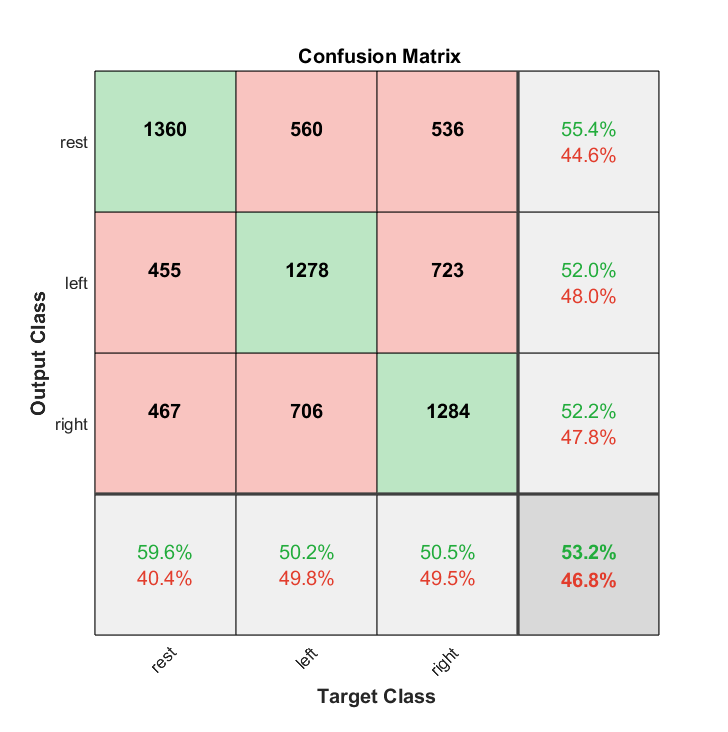
\includegraphics[width=0.8\linewidth]{slike/ConfusionSVM.png}
    \end{center}
    \caption[Matrika zmede metode Quadratic SVM.]{Matrika zmede metode Quadratic SVM. V poljih vidno število stanj. Od zgoraj navzdol: stanje mirovanja, skrčena leva pest, skrčena desna pest.}
    \label{slika:SVM_matrika}
    \end{figure}

\subsection{Rezultati z uporabo lastne nevronske mreže}
Nato smo poskusili z zgoraj navedeno nevronsko mrežo, ki razvršča matrike povezljivosti. Mreža je dosegla enako točnost kot metode iz aplikacije Clasification Learner in sicer 52\%. Če primerjamo matriko zmede nevronske mreže z matriko zmede metode SVM (sliki \ref{slika:nevronska_mreza_matrika} in \ref{slika:SVM_matrika} ), opazimo, da obe metodi bolj natančno razlikujeta stanje mirovanja od obeh stanj gibanja, medtem ko je razlikovanje med stanji gibanja med seboj manj natančno.

\begin{figure}
\begin{center}
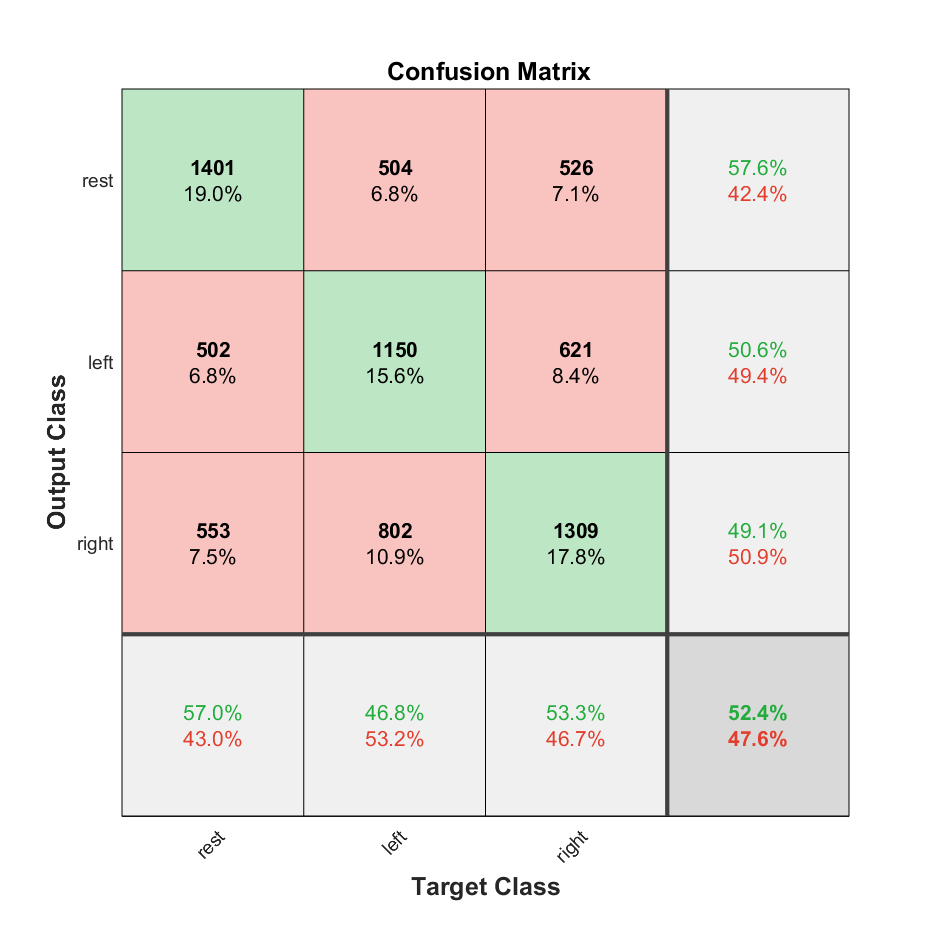
\includegraphics[width=0.8\linewidth]{slike/Confusion_13-20Hz_0s-4s.png}
\end{center}
\caption[Matrika zmede lastne nevronske mreže.]{Matrika zmede lastne nevronske mreže. V zelenih poljih vidna točnost za posamezna stanja. Od zgoraj navzdol: stanje mirovanja, skrčena leva pest, skrčena desna pest.}
\label{slika:nevronska_mreza_matrika}
\end{figure}



\section{Rezultati na lastnih podatkih}
Da bi se približali delovanju v realnem času, smo nevronsko mrežo dodatno naučili na naših podatkih. Zaradi različnih pogojev snemanja in natančnosti naprav, na katerih so podatki bili posneti, točnost razvrščanja pričakovano padla. Dosegli smo 43\% točnost. Ker nimamo velikega števila posnetkov smo uporabili petkratno prečno preverjanje. 
\begin{figure}
\begin{center}
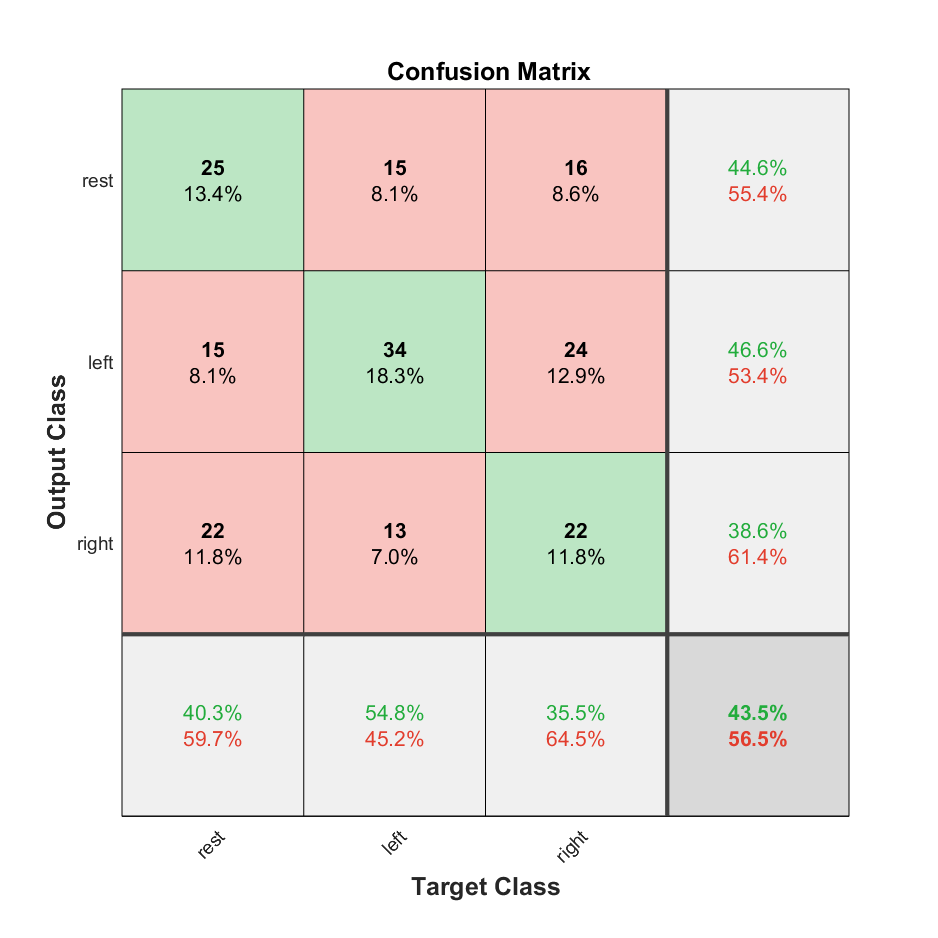
\includegraphics[width=0.8\linewidth]{slike/Confusion_13-20Hz_0s-4s_retrained.png}
\end{center}
\caption[Matrika zmede dodatno naučene nevronske mreže.]{Matrika zmede nevronskih mrež dodatno naučenih na naših podatkih.}
\end{figure}


\section{Sprotno razpoznavanje}
Po razvoju pristopov na zbirkah podatkov smo implementirali sprotno razpoznavanje. Za prenos podatkov iz naprave Quick-20 v okolje MATLAB smo uporabili programsko opremo Lab Streaming Layer. V okolju MATLAB smo podatke združevali in iz njih vsako sekundo izračunali matriko povezljivosti z metodo CPCC za frekvenčno območje beta, filtrirano z Butterwithovim filtrom. Matriko povezljivosti smo razvrstili in rezultat razvrščanja izpisali na zaslon. Na natančnost sprotnega razvrščanja matrik povezljivosti ene osebe vpliva veliko dejavnikov. Nanj vpliva razpoloženje osebe, namestitev naprave, sam dogodek, ki ga razvrščamo, pa tudi motnje v okolju, ki vplivajo na osebo in napravo. Točnosti razvrščanj nismo natančno izmerili, ocenjujemo pa, da je nižja od tiste, ki smo jo dosegli na prej posnetih podatkih. Kljub temu je iz rezultatov razvidno, da je klasifikacija gibanja v realnem času mogoča.

\begin{figure}
    \begin{center}
    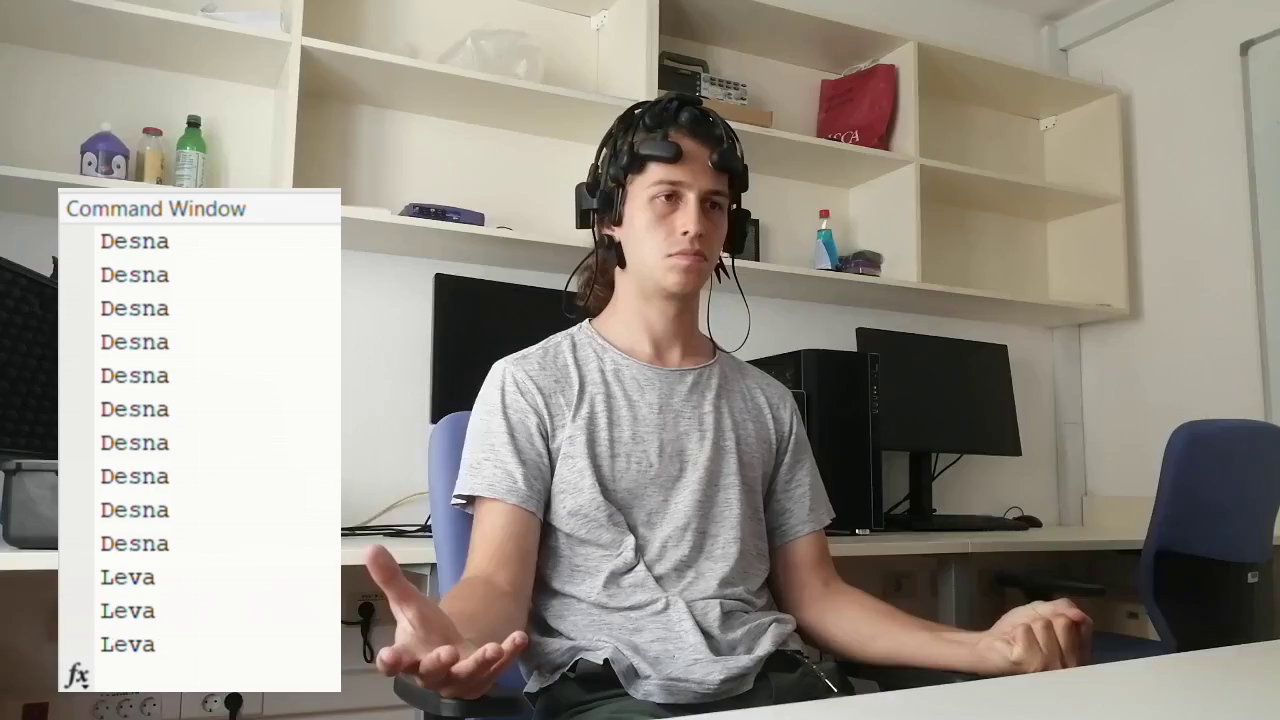
\includegraphics[width=1\linewidth]{slike/razpoznavanje.png}
    \end{center}
    \caption[Prikaz sprotnega razpoznavanja]{Prikaz sprotnega razpoznavanja. Dodan izpis razvrščanja iz okolja MATLAB.}
    \end{figure}



